%%\def\beginanswers{\iffalse}
\def\beginanswers{\iftrue}

\documentclass[10pt]{article}
\usepackage{amsmath,amsfonts,amsthm,amssymb}
\usepackage{graphicx}
\usepackage{enumerate}
\usepackage{upquote,textcomp}
\usepackage{listings}
\usepackage{color}

\definecolor{mygreen}{rgb}{0,0.6,0}
\definecolor{mygray}{rgb}{0.5,0.5,0.5}
\definecolor{mymauve}{rgb}{0.58,0,0.82}


\lstset{frame=tb,
  language=,
  aboveskip=3mm,
  belowskip=3mm,
  showstringspaces=false,
  columns=flexible,
  keepspaces=true,
  basicstyle={\small\ttfamily},
  numbers=none,
  numberstyle=\tiny\color{black},
  keywordstyle=\color{black},
  commentstyle=\color{black},
  stringstyle=\color{black},
  breaklines=true,
  breakatwhitespace=true,
  tabsize=3
}

\lstset{frame=tb,
  language=Python,
  aboveskip=3mm,
  belowskip=3mm,
  showstringspaces=false,
  columns=flexible,
  basicstyle={\small\ttfamily},
  numbers=none,
  numberstyle=\tiny\color{mygray},
  keywordstyle=\color{blue},
  commentstyle=\color{mygreen},
  stringstyle=\color{mymauve},
  breaklines=true,
  breakatwhitespace=true,
  tabsize=3
}


\newcommand{\vect}[1]{{\bf #1}}                 %for bold chars
\newcommand{\vecg}[1]{\mbox{\boldmath $ #1 $}}  %for bold greek chars
\newcommand{\matx}[1]{{\bf #1}}

\setlength{\parindent}{0in}
\setlength{\parskip}{1em}
\setlength{\textheight}{9.5in}
\setlength{\textwidth}{7in}
\setlength{\headsep}{0in}        % distance from top of page to address
\setlength{\topmargin}{-0.5in}
\setlength{\oddsidemargin}{-0.5in}
\setlength{\evensidemargin}{-0.5in}


\begin{document}
\thispagestyle{empty}

\vspace*{0.5in}

\begin{center}
\Large
\textbf{Open Source Software --- CSCI-4470 --- Spring 2021} \\
\textbf{Test 1} \\
\textbf{March 5, 2021}
\end{center}


%%%%%%%%%%%%%%%%%%%%%%%%%%%%%%%%%%%%%%%%%%%%%%%%%%%%%%%%%%%%%%%%%%%%%%%%
%%%%%%%%%%%%%%%%%%%%%%%%%%%%%%%%%%%%%%%%%%%%%%%%%%%%%%%%%%%%%%%%%%%%%%%%
\beginanswers
\begin{center}
\Large
\textbf{SOLUTIONS}
\end{center}

%%%%%%%%%%%%%%%%%%%%%%%%%%%%%%%%%%%%%%%%%%%%%%%%%%%%%%%%%%%%%%%%%%%%%%%%
\else
%%%%%%%%%%%%%%%%%%%%%%%%%%%%%%%%%%%%%%%%%%%%%%%%%%%%%%%%%%%%%%%%%%%%%%%%


\begin{center}

\textbf{\Large Name:} \underline {\hspace{2.0in}} \\

\bigskip
\bigskip

\centerline{
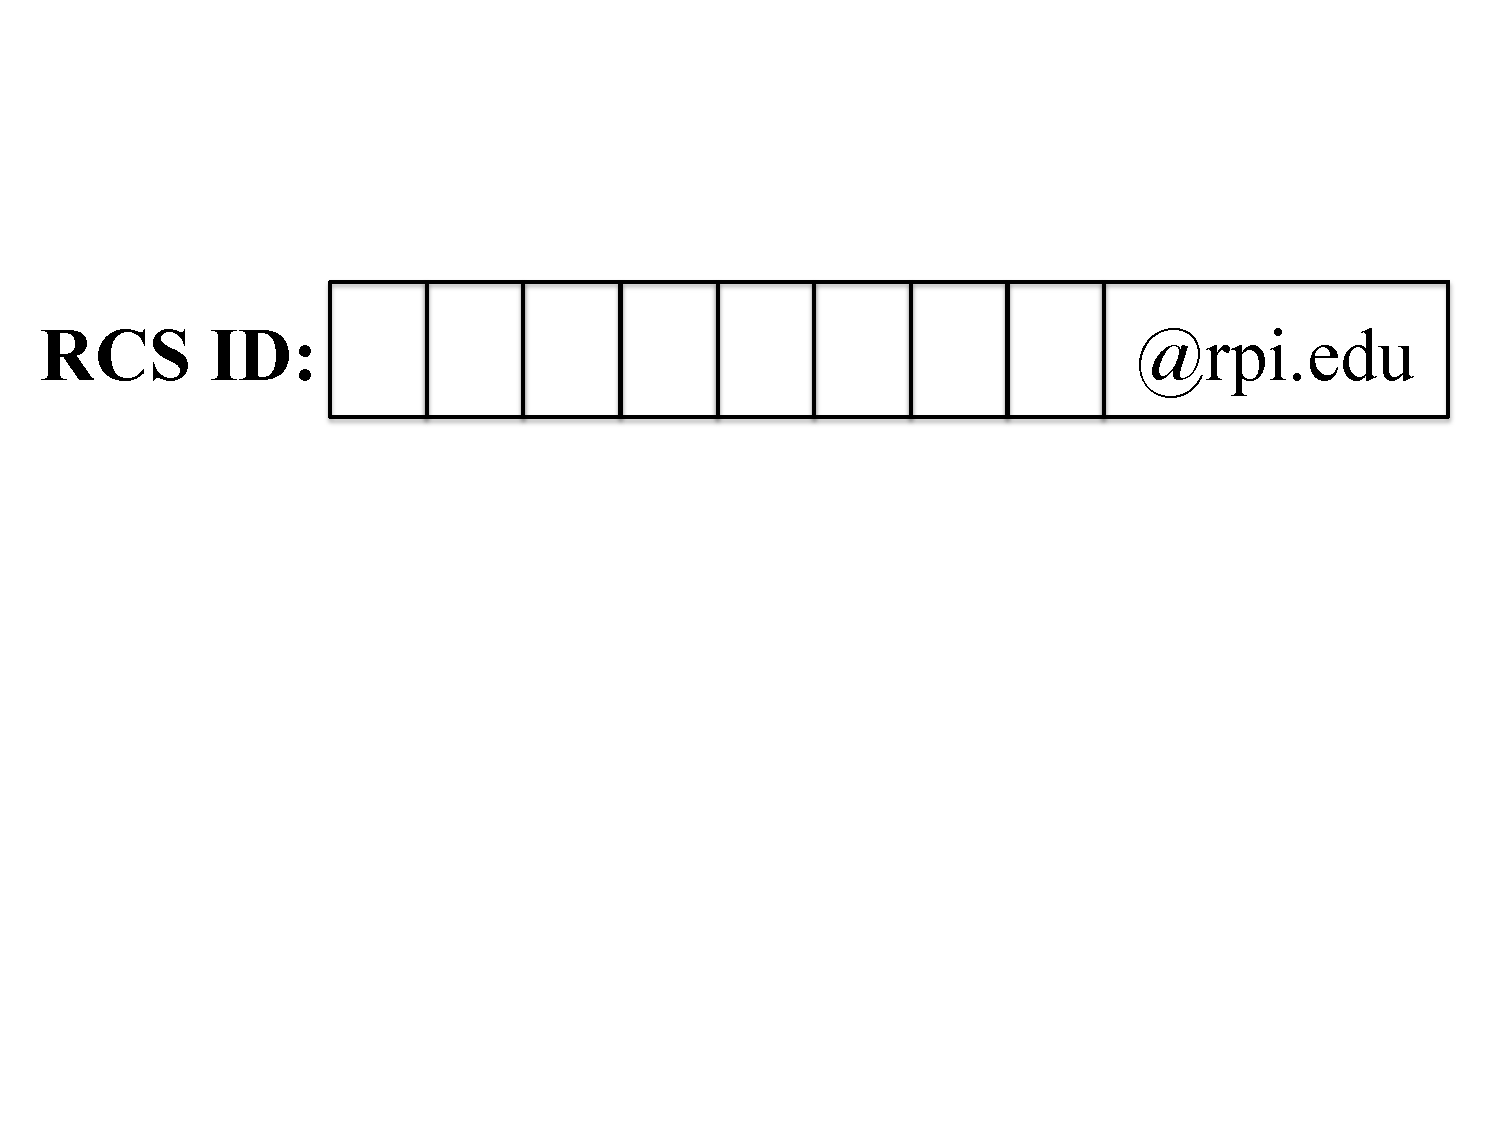
\includegraphics[height=0.5in]{boxes}
}

%%  \begin{tabular}{|p{0.1in}|p{0.1in}|p{0.1in}|p{0.1in}|p{0.1in}|p{0.1in}|p{0.1in}|p{0.1in}|l|}
%%    \hline \\
%%   & & & & & & & & \textbf{\large @rpi.edu} \\
%%  \hline
%%  \end{tabular} 
%%  
%%  \end{tabular}

\bigskip

\textbf{\Large RIN\#:} \underline {\hspace{1.5in}}  

\vspace*{0.4in}
{\large\bf Honor pledge: On my honor I have neither given
nor received aid on this exam.}

\vspace*{0.1in}
{\large\bf Please sign here to indicate that you agree with the honor pledge: \underline {\hspace{1.5in}}}
\end{center}

\vspace*{.45in} 

{\large\bf Instructions:}
\begin{itemize}
%%\item You have 90 minutes to complete this test.
\item Clearly print your name, RCS ID (in all caps.) and your RIN at the top of your exam.
\item This test is open book, open notes and open computer. You {\textbf may not} use the internet. Please turn off your wifi.
\item There are \textbf{6 questions} on this test worth a total of
  \textbf{100 points}.
\end{itemize}

\centering{\begin{tabular}{|c|c|r|}
	\hline
	Question & Score & Possible \\ \hline
	1 &  & 10 \\ \hline
	2 &  & 12 \\ \hline
	3 &  & 18 \\ \hline
	4 &  & 16 \\ \hline
	5 &  & 20 \\ \hline
	6 &  & 24 \\ \hline
	Total &  & 100 \\ \hline
\end{tabular}}

\newpage

%% ^\d?[\( ]?(\d{3})[- \)]*\d{3}[- \)]*\d{4}

%%%%%%%%%%%%%%%%%%%%%%%%%%%%%%%%%%%%%%%%%%%%%%%%%%%%%%%%%%%%%%%%%%%%%%%%
\fi
%%%%%%%%%%%%%%%%%%%%%%%%%%%%%%%%%%%%%%%%%%%%%%%%%%%%%%%%%%%%%%%%%%%%%%%%

\begin{enumerate}
	%% Spring 2021
	\item Given the following regex expression (10pts):
	
	 \verb+\( (\d*)\)\:\s*at \w*\.\w*\.(\w*)\((\w*\.\w*)\:(\d*)\)+
	 
	 indicate the values of the 5 capture groups when applied to the string:
	 
	  \verb+E/( 1553):   at widget.List.fillDown(ListView.java:652)+
	\beginanswers
		\begin{enumerate}[1]
		\bigskip
		\item 1553
		\bigskip
		\item fillDown
		\bigskip
		\item ListView.java
		\bigskip
		\item 652
		\bigskip
		\item \verb|<There are only 4>|
		\bigskip
		\end{enumerate}
	\else
		
		\begin{enumerate}[1]
		\bigskip
		\item Capture Group 1	
		\bigskip
		\bigskip
	\bigskip
	\bigskip
		\bigskip
	\bigskip
	\bigskip
		\bigskip
		\bigskip
		\item Capture Group 2
		\bigskip
		\bigskip
	\bigskip
	\bigskip
		\bigskip
	\bigskip
	\bigskip
		\bigskip
		\bigskip
		\item Capture Group 3
		\bigskip
		\bigskip
	\bigskip
\bigskip
\bigskip
	\bigskip
\bigskip
\bigskip
		\bigskip
		\item Capture Group 4
		\bigskip
		\bigskip
		\bigskip
	\bigskip
	\bigskip
		\bigskip
	\bigskip
	\bigskip
		\bigskip
		\item Capture Group 5
		\bigskip
		\bigskip
		\bigskip
	\bigskip
	\bigskip
		\bigskip
	\bigskip
	\bigskip
		\bigskip
		\end{enumerate}
		\fi
	
\newpage


	\item The Booz Allen Public License v1.0 reads in part:
	
	\begin{quote}
		\textbf{Government/Non-Profit Academic/Other Non-Profit.}
		This Section applies if You are not a Commercial Entity.
		
		\begin{itemize}
			\item \textbf{License.} Subject to the terms and conditions of this License, each Originator hereby grants You a perpetual, worldwide, non-exclusive, royalty-free license to reproduce, display, perform, modify, distribute and otherwise use the Product and Derivatives, in Source Code and Object Code form, in accordance with the terms and conditions of this License in order to support the general public good and for your internal business purposes.
		
			\item \textbf{Distribution.} You may distribute to third parties copies of the Product, including any Derivative that You create, in Source Code or Object Code form. If You distribute copies of the Product, including any Derivative that You create, in Source Code form, such distribution must be under the terms of this License and You must inform recipients of the Source Code that the Product is governed under this License and how they can obtain a copy of this License. You may distribute to third parties copies of the Product, including any Derivative that You create, in Object Code form, or allow third parties to access or use the Product, including any Derivative that You create, under a license of Your choice.
		
   			\item \textbf{Commercial Sales.} You may not distribute, or allow third parties to access or use, the Product or any Derivative for a fee, unless You first obtain permission from the Originator. If Booz Allen Hamilton is the Originator, please contact Booz Allen Hamilton at opensource@bah.com.
	\end{itemize}	
	
		\textbf{Commercial Entities.}
		This Section applies if You are a Commercial Entity.
		
		\begin{itemize}
		\item \textbf{License.} Subject to the terms and conditions of this License, each Originator hereby grants You a perpetual, worldwide, non-exclusive, royalty-free license to reproduce, display, perform, modify, distribute and otherwise use the Product and Derivatives, in Source Code and Object Code form, in accordance with the terms and conditions of this License for the sole purpose of Your internal business purposes and the provision of services to government, non-profit academic, and other non-profit entities.
		
		\item \textbf{Distribution and Derivatives.} You may distribute to third parties copies of the Product, including any Derivative that You create, in Source Code or Object Code form. If You distribute copies of the Product, including any Derivative that You create, in Source Code form, such distribution must be under the terms of this License and You must inform recipients of the Source Code that the Product is governed under this License and how they can obtain a copy of this License. You may distribute to third parties copies of the Product, including any Derivative that You create, in Object Code form, or allow third parties to access or use the Product, including any Derivative that You create, under a license of Your choice, provided that You make available, and inform the recipient of such distribution how they can obtain, a copy of the Source Code thereof, at no charge, and inform the recipient of the Source Code that the Product is governed under this License and how they can obtain a copy of this License.
		
		\item Commercial Sales. You may not distribute, or allow third parties to access or use, the Product or any Derivative for a fee, unless You first obtain permission from the Originator. If Booz Allen Hamilton, please contact Booz Allen Hamilton at opensource@bah.com.
		\end{itemize}
	\end{quote}

	It clearly is in conflict with at least 2 of the 10 criteria in the Open Source Definiton. Identify 2 criteria which it is in conflict with and explain your reasoning.  (12 pts)
 
 \newpage
 	
\beginanswers
\begin{enumerate}[1]
	\item \textbf{Clause:} Free Redistribution (Clause 1)
	
	\item \textbf{Reasoning:} Free redistribution implies the right to sell. Open source licenses cannot require additional permissions from the originator in order to exercise this right.
	
	\item \textbf{Clause:} No Discrimination Against Fields of Endeavor (Clause 5)
	
	\item \textbf{Reasoning:} Granting one set of rights to commercial and a different set of rights to non-commercial and government is a clear discrimination against  field of endeavor.
	
\end{enumerate}
\newpage
\else
\begin{enumerate}[1]
	\item \textbf{Clause: (3 pts.)} 
	\bigskip
	\bigskip
	\bigskip
	\bigskip
\bigskip
\bigskip
	\bigskip
	\bigskip
	\bigskip
	\item \textbf{Reasoning: (3pts)}
	\bigskip
	\bigskip
	\bigskip
\bigskip
\bigskip
	\bigskip
	\bigskip
	\bigskip
	\bigskip
	\item \textbf{Clause: (3pts)}
	\bigskip
	\bigskip
	\bigskip
	\bigskip
	\bigskip
\bigskip
\bigskip
	\bigskip
	\bigskip
	\item \textbf{Reasoning: (3pts)}
	\bigskip
	\bigskip
	\bigskip
	\bigskip
\bigskip
\bigskip
	\bigskip
	\bigskip
	\bigskip
\end{enumerate}
\fi

\newpage

    \item For each of the following document constructs, show how to create them using different documentation tools we covered in class (18 pts):
    
    \begin{enumerate}
    	\item A bulleted list of three items such as:
    	\begin{itemize}
    		\item Item 1
    		\item Item 2
    		\item Item 3
    	\end{itemize}
    \beginanswers
    \begin{enumerate}
    	\item MarkDown:
    	\begin{verbatim}
* Item 1
* Item 2
* Item 3
    	\end{verbatim}

    	\item reStructuredText
		\begin{verbatim}
* Item 1
* Item 2
* Item 3
		\end{verbatim}

    	\item LaTex
    	\begin{verbatim}
\begin{itemize}
	\item Item 1
	\item Item 2
	\item Item 3
\end{itemize}
    	\end{verbatim}
    	
    \end{enumerate}
	\else
    \begin{enumerate}
   \item MarkDown
\bigskip
	\bigskip
\bigskip
	\bigskip
\bigskip
\bigskip
\bigskip
     	\item reStructuredText
	\bigskip
	\bigskip
\bigskip
\bigskip
\bigskip
\bigskip
\bigskip
    	\item LaTex
	\bigskip
\bigskip
	\bigskip
\bigskip
\bigskip
\bigskip
\bigskip
	\end{enumerate}
	\fi

\item A hyperlink to the OSI website with a clickable link \verb*|OSI| that points to \verb*|https://opensource.org/|
    \beginanswers
\begin{enumerate}
	\item MarkDown:
	\begin{verbatim}
		[OSI](https://opensource.org/)
	\end{verbatim}
	
	\item reStructuredText
	\begin{verbatim}
		`OSI <https://opensource.org/>`_
	\end{verbatim}
	
	\item HTML
	\begin{verbatim}
		<a href=https://opensource.org/>OSI</a>
	\end{verbatim}
	
\end{enumerate}
\else
\begin{enumerate}
	\item MarkDown
	\bigskip
	\bigskip
	\bigskip
	\bigskip
	\bigskip
	\bigskip
	\bigskip
	\item reStructuredText
	\bigskip
	\bigskip
	\bigskip
	\bigskip
	\bigskip
	\bigskip
	\bigskip
	\item HTML
	\bigskip
	\bigskip
	\bigskip
	\bigskip
	\bigskip
	\bigskip
	\bigskip
\end{enumerate}
\fi

\newpage

\end{enumerate}

\item Provide answers to the questions below. Your answers do not need to be long. A few sentences should be sufficient to capture the important points (16pts).

\begin{enumerate}
	\item In class we covered why formats like MarkDown and reStructuredText as well as Literate Programming are especially important for open source projects. Discuss why below. 
	
	\beginanswers
	Open source projects require that the source code be part of the data a user has access to. By using open, text based formats we allow our documentation to be embedded with the code without requiring special proprietary programs to allow it to be read and understood. A user with access to the source can get access to the author documentation as well and the documentation can be maintained using the same tools as the source code including issue trakers and pull requests. Literate programming takes this a step further by embedding the code directly in the same document as the code description and possibly the design.
	\else
	\bigskip
	\bigskip
	\bigskip
	\bigskip
	\bigskip
	\bigskip
	\bigskip
	\bigskip
	\bigskip
	\bigskip
\bigskip
\bigskip
\bigskip
\bigskip
\bigskip
\bigskip
\bigskip
\bigskip
\bigskip
\bigskip
	\fi

	\item Discuss the importance of a license on an open source repository. Make sure to address what happens to your rights to use the code when a copyright holder changes the license used.

	\beginanswers
Copyright is granted at the time a piece of art is created and doesn't require additional marking so any code without an explicit license should be considered proprietary. Alicense is the way you ensure that you have the rights to use a piece of code and for what purposes, or conversely is the way you guarantee to the members of your community the way they are allowed to use your code. A copyright holder can change the license on their code to anything including proprietary, however, this only affects versions of the code from that point in time forward. They cannot retroactively remove rights they granted to you in previous versions, so all code acquired under the prevous license can still be used under the previous terms.
\else
\bigskip
\bigskip
\bigskip
\bigskip
\bigskip
\bigskip
\bigskip
\bigskip
\bigskip
\bigskip
\bigskip
\bigskip
\bigskip
\bigskip
\bigskip
\bigskip
\bigskip
\bigskip
\bigskip
\bigskip
\fi
\end{enumerate}
	
\newpage


\item Consider the following scenario. You have an empty remote repository on github at
\begin{verbatim}
	git@github.com:username/project.git
\end{verbatim} 

You also have a  project on your local computer that represents your new repository. Your directory already has files: \verb|README.md| file. Give the sequence of commands to create the repository on your local system, set the remote \verb|origin| to be your remote reposiitory and get the file \verb*|README.md| in both the local and remote. You must use the command line for all git operations. (20 pts)

Write your git commands below

\beginanswers
\begin{lstlisting}
git init
git remote add origin git@github.com:username/project.git
git add README.md 
git commit -m "Initial Commit"
git push --set-upstream origin master
\end{lstlisting}
\else
\hspace*{-0.4in}\framebox(540,460){}
\fi
\newpage

\item Assume you have the following files in your current directory: (24pts):

\begin{itemize}
	\item \verb*|main.c|
	\item \verb*|helper.h| and \verb*|helper.c|
	\item \verb*|shared/shared.h| and \verb*|shared/shared.c|
	\item \verb*|static/static.h| and \verb*|static/static.c|
	\item \verb*|helper.c| depends on \verb*|shared/shared.c| and \verb*|static/static.c|
	\item \verb*|main.c| depends on \verb*|helper.c|
\end{itemize}

\begin{enumerate}
\item Write a \verb*|Makefile| that captures this relationship to create the executable \verb*|main.exe|.  (14 of 24 pts).

A few notes:
\begin{itemize}
	\item \verb*|shared/shared.c| must go into the shared library \verb*|libshared.so|
	\item \verb*|static/static.c| must go into the shared library \verb*|libstatic.a|
	\item Do not use shortcuts. Put in the commands to create each object file and each library, etc. explicitly in the file.
	\item The \verb*|Makefile| must be hand generated. Do not use a Makefile generator (such as cmake) to create the file.
	\item Make sure you have a \verb*|clean| target that removes all of the files you generate.
\end{itemize}
\beginanswers
\begin{lstlisting}[language=make]
all: main

clean:
	rm main.o helper.o static.o shared.o main libstatic.a libshared.so

main.o: main.c helper.h
	cc -c -o main.o main.c

helper.o: helper.c helper.h static/static.h shared/shared.h
	cc -c -o helper.o helper.c

static.o: static/static.c static/static.h
	cc -c -o static.o static/static.c

shared.o: shared/shared.c shared/shared.h
	cc -fPIC -c shared/shared.c -o shared.o

main: main.o helper.o helper.h libstatic.a libshared.so
	cc main.o helper.o libstatic.a libshared.so -o main -Wl,-rpath .

libstatic.a: static.o
	ar qc libstatic.a static.o

libshared.so: shared.o
	cc -shared -o libshared.so shared.o
\end{lstlisting}
\else
\hspace*{-0.4in}\framebox(540,400){}
\fi
\newpage
	\item Now turn the Makefile into a CMakeLists.txt file. Add the commands to generate an install target to install ``main.exe''  ``bin'' and the shared library into ``lib'' (10 of 24 pts):

\beginanswers
\begin{lstlisting}[language=make]
cmake_minimum_required(VERSION 3.0)
project(Main C)

add_library(shared SHARED shared/shared.c)

add_library(static STATIC static/static.c)

add_executable(main main.c helper.c)
target_link_libraries(main shared static)

install(TARGETS shared DESTINATION lib)
install(TARGETS main DESTINATION bin)
\end{lstlisting}
\else

\textbf{CMakeLists.txt}:

\hspace*{-0.4in}\framebox(540,400){}

\fi
\end{enumerate}
	
\end{enumerate}
\end{document}
